\ifspanish
TBD
\else

Let ${X_k, k \ge 0}$ be a Markov chain with state space ${\cal Z} = \{0, 1, 2\}$ and the transition graph shown in the figure.
\begin{center}
\centering
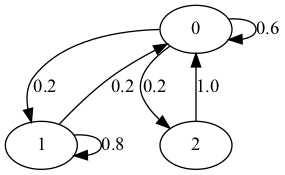
\includegraphics[width=0.25\textwidth]{./db/figs/MC_2023.png}
\end{center}

\begin{parts}
\part Show the transition matrix
\part Compute $P\{X_{22} = 1 | X_{20}=2\}$
\part Compute the stationary distribution.
\end{parts}

\begin{solution}
\begin{parts}
\part 
\begin{align*}
{\bf P} = 
	\begin{pmatrix}
	0.6 & 0.2 & 0.2   \\
	0.2 & 0.8 & 0     \\
	1   & 0   & 0 	
	\end{pmatrix}
\end{align*}
\part 
\begin{align*}
P\{X_{22} = 1| X_{20} = 2\} = 
	\begin{pmatrix} 0 & 1 & 0 \end{pmatrix}
	{\bf P}^\intercal
	{\bf P}^\intercal
	\begin{pmatrix} 0 \\ 0 \\ 1 	\end{pmatrix}
	=
	\begin{pmatrix} 0.2 & 0.8 & 0 \end{pmatrix}
	\begin{pmatrix} 1 \\ 0 \\ 0 \end{pmatrix}
	= 0.2
\end{align*}

\part This is the solution of
\begin{align*}
\begin{pmatrix}
{\bf P}^\intercal - {\bf I}  \\
\mathbb{1}^\intercal   
\end{pmatrix}
\bm{\pi} = 
\begin{pmatrix} 0 \\ 0 \\ 0 \\ 1 \end{pmatrix}
\end{align*}
that is
\begin{align*}
\begin{pmatrix}
-0.4 &  0.2 &  0.2  \\
 0.2 & -0.2 &  0    \\
 0.2 &  0   & -1    \\
 1   &  1   &  1
\end{pmatrix}
\bm{\pi} = 
\begin{pmatrix} 0 \\ 0 \\ 0 \\ 1 \end{pmatrix}
\end{align*}
which, removing the first row (which is redundant), reduces to
\begin{align*}
\begin{pmatrix}
0.2  & -0.2 &  0    \\
0.2  & 0    & -1    \\
1    & 1    &  1
\end{pmatrix}
\bm{\pi} = 
\begin{pmatrix} 0 \\ 0 \\ 1 \end{pmatrix}
\end{align*}
whose solution is
\begin{align*}
\bm{\pi} = 
\frac{1}{11} \begin{pmatrix} 5 \\ 5 \\ 1 \end{pmatrix}
\end{align*}

 \end{parts}
\end{solution}

\fi
